\section{Buttons/Switches}


\subsection{Objectives}
In this lab, you will
\begin{itemize}
    \item Learn how to add new C source files and C header files in an STM32 project, 
    \item Learn how to read digital inputs and display values to LEDs using a timer interrupt of a microcontroller (MCU). 
    \item Learn how to debounce when reading a button.
    \item Learn how to create an FSM and implement an FSM in an MCU.
\end{itemize}

\subsection{Introduction}
Embedded systems usually use buttons (or keys, or switches, or any form of mechanical contacts) as part of their user interface. This general rule applies from the most basic remote-control system for opening a garage door, right up to the most sophisticated aircraft autopilot system. Whatever the system you create, you need to be able to create a reliable button interface. 

%add a picture of buttons/switch

A button is generally hooked up to an MCU so as to generate a certain logic level when pushed or closed or ``active" and the opposite logic level when unpushed or open or ``inactive."  The active logic level can be either `0' or `1', but for reasons both historical and electrical, an active level of '0' is more common.

We can use a button if we want to perform operations such as:
\begin{itemize}
    \item Drive a motor while a switch is pressed.
    \item Switch on a light while a switch is pressed.
    \item Activate a pump while a switch is pressed.
\end{itemize}
These operations could be implemented using an electrical button without using an MCU; however, use of an MCU may well be appropriate if we require more complex behaviours. For example:
\begin{itemize}
    \item Drive a motor while a switch is pressed. 
    
    \textbf{Condition}: If the safety guard is not in place, don't turn the motor. Instead sound a buzzer for 2 seconds. 
    \item Switch on a light while a switch is pressed.
    
    \textbf{Condition}: To save power, ignore requests to turn on the light during daylight hours. 
    
    \item Activate a pump while a switch is pressed
    
    \textbf{Condition}: If the main water reservoir is below 300 litres, do not start the main pump: instead, start the reserve pump and draw the water from the emergency tank. 
\end{itemize}

In this lab, we consider how you read inputs from mechanical buttons in your embedded application using an MCU. 

% Before considering button/switches themselves, we will consider the process of reading the state of port pins.
\newpage
\subsection{Basic techniques for reading from port pins}
\subsubsection{The need for pull-up resistors}
\begin{figure}[!htp]
    \centering
    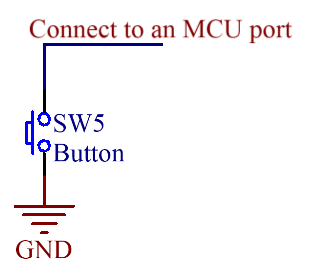
\includegraphics[width=2in]{source/picture/bai_3/Button_Schematic_0.png}
    \caption{\textit{Connecting a button to an MCU}}
    \label{bai4_pic_button_schematic_0}
\end{figure}
Figure \ref{bai4_pic_button_schematic_0} shows a way to connect a button to an MCU. This hardware operates as follows:
\begin{itemize}
    \item When the switch is open, it has no impact on the port pin. An internal resistor on the port ``pulls up" the pin to the supply voltage of the MCU (typically 3.3V for STM32F103). If we read the pin, we will see the value `1'. 
    \item When the switch is closed (pressed), the pin voltage will be 0V. If we read the pin, we will see the value `0'. 
\end{itemize}
 
 However, if the MCU does not have a pull-up resistor inside, when the button is pressed, the read value will be `0', but even we release the button, the read value is still `0' as shown in Figure \ref{bai4_pic_the_need_of_pull_up_resistors}.
 \begin{figure}[!htp]
    \centering
    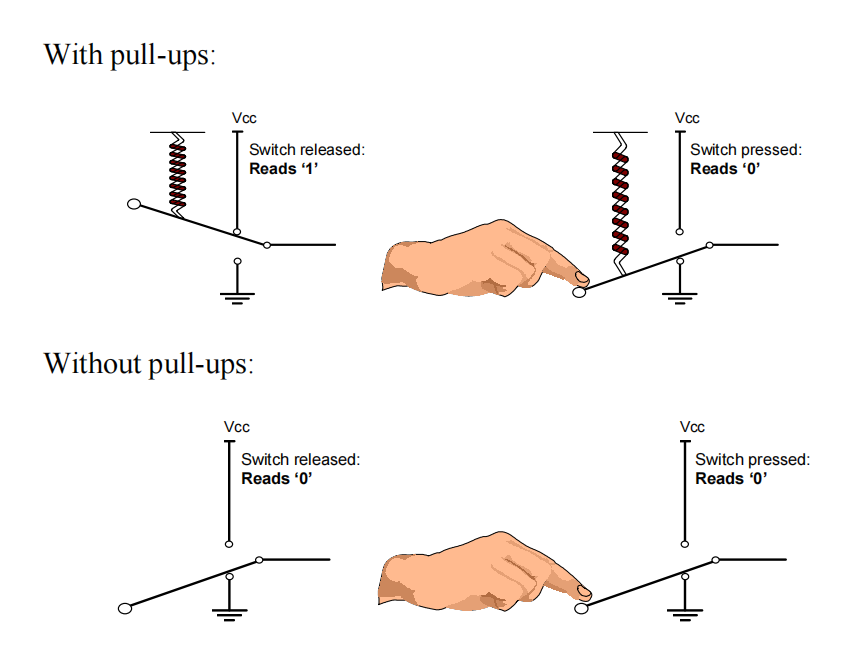
\includegraphics[width=4.5in]{source/picture/bai_3/pullup_resistors.png}
    \caption{\textit{The need of pull up resistors}}
    \label{bai4_pic_the_need_of_pull_up_resistors}
\end{figure}
%add a picture 

So a reliable way to connect a button/switch to an MCU is that we explicitly use an external pull-up resistor as shown in Figure \ref{bai4_pic_button_schematic_1}.

 \begin{figure}[!htp]
    \centering
    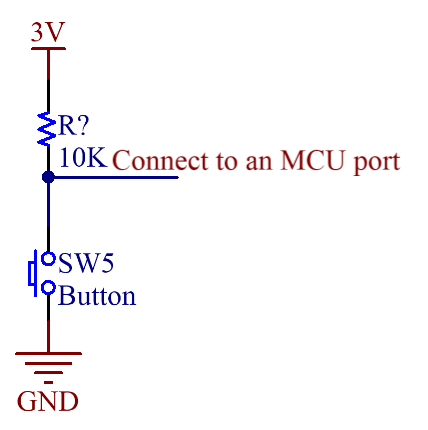
\includegraphics[width=2in]{source/picture/bai_3/Button_Schematic.png}
    \caption{\textit{A reliable way to connect a button to an MCU}}
    \label{bai4_pic_button_schematic_1}
\end{figure}
 
%\newpage 
\subsubsection{Dealing with switch bounces}
In practice, all mechanical switch contacts bounce (that is, turn on and off, repeatedly, for short period of time) after the switch is closed or opened as shown in Figure \ref{bai4_pic_switchsbounce}.
\begin{figure}[!htp]
    \centering
    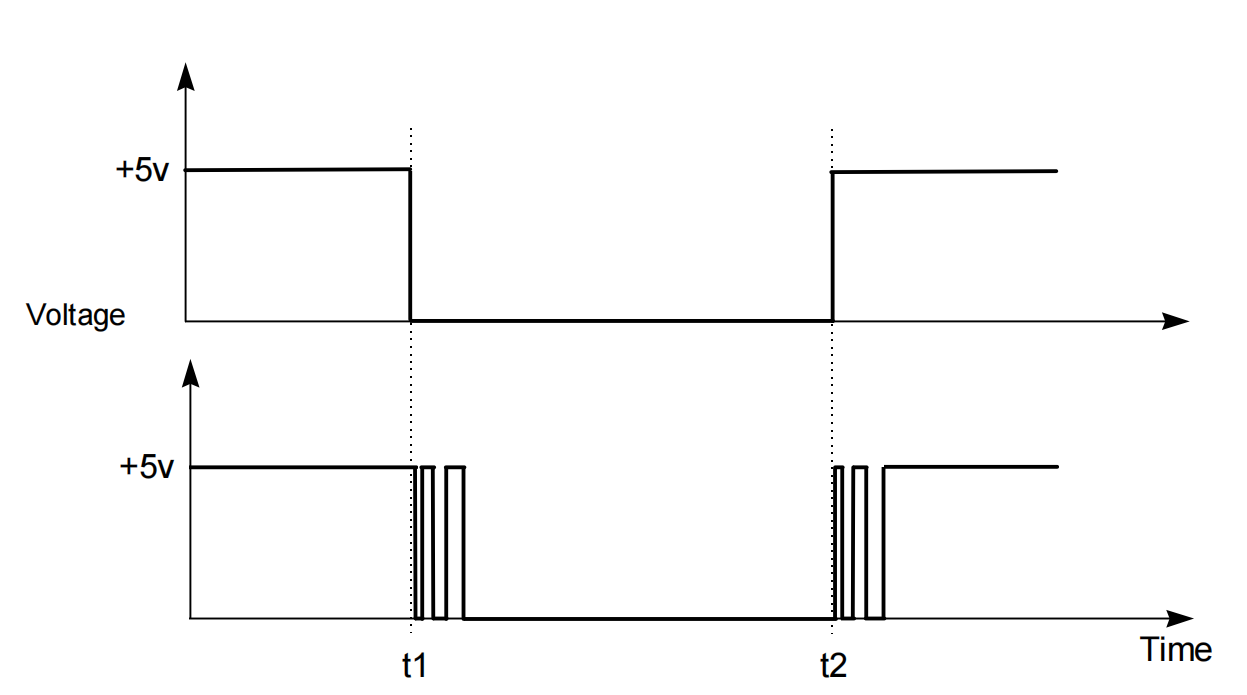
\includegraphics[width=4.5in]{source/picture/bai_3/switchsbounce.png}
    \caption{\textit{Switch bounces}}
    \label{bai4_pic_switchsbounce}
\end{figure}

Every system that uses any kind of mechanical switch must deal with the issue of debouncing.  The key task is to make sure that one mechanical switch or button action is only read as one action by the MCU, even though the MCU will typically be fast enough to detect the unwanted switch bounces and treat them as separate events.  Bouncing can be eliminated by special ICs or by RC circuitry, but in most cases debouncing is done in software because software is ``free".

As far as the MCU concerns, each ``bounce" is equivalent to one press and release of an ``ideal” switch. 
Without appropriate software design, this can give several problems:
\begin{itemize}
    \item Rather than reading ‘A’ from a keypad, we may read ‘AAAAA’
    \item Counting the number of times that a switch is pressed becomes extremely difficult
    \item If a switch is depressed once, and then released some time later, the `bounce' may make it appear as if the switch has been pressed again (at the time of release). 
\end{itemize}


The key to debouncing is to establish a minimum criterion for a valid button push, one that can be implemented in software.  This criterion must involve differences in time - two button presses in 20ms must be treated as one button event, while two button presses in 2 seconds must be treated as two button events.  So what are the relevant times we need to consider?  They are these:
\begin{itemize}
    \item Bounce time:  most buttons seem to stop bouncing within 10ms
    \item Button press time: the shortest time a user can press and release a button seems to be between 50 and 100ms
    \item Response time: a user notices if the system response is 100ms after the button press, but not if it is 50ms after
\end{itemize}



Combining all of these times, we can set a few goals
\begin{itemize}
    \item Ignore all bouncing within 10ms
    \item Provide a response within 50ms of detecting a button push (or release)
    \item Be able to detect a 50ms push and a 50ms release    
\end{itemize}


The simplest debouncing method is to examine the keys (or buttons or switches) every N milliseconds, where N > 10ms (our specified button bounce upper limit) and N <= 50ms (our specified response time).   We then have three possible outcomes every time we read a button:
\begin{itemize}
    \item We read the button in the solid `0' state
    \item We read the button in the solid `1' state
    \item We read the button while it is bouncing (so we will get either a `0' or a `1')
\end{itemize}

Outcomes 1 and 2 pose no problems, as they are what we would always like to happen.  Outcome 3 also poses no problem because during a bounce either state is acceptable.  If we have just pressed an active-low button and we read a '1' as it bounces, the next time through we are guaranteed to read a '0' (remember, the next time through all bouncing will have ceased), so we will just detect the button push a bit later.  Otherwise, if we read a '0' as the button bounces, it will still be '0' the next time after all bouncing has stopped, so we are just detecting the button push a bit earlier.  The same applies to releasing a button.  Reading a single bounce (with all bouncing over by the time of the next read) will never give us an invalid button state.  It's only reading multiple bounces (multiple reads while bouncing is occurring) that can give invalid button states such as repeated push signals from one physical push. 

So if we guarantee that all bouncing is done by the time we next read the button, we're good.  Well, almost good, if we're lucky...

MCUs often live among high-energy beasts, and often control the beasts.  High energy devices make electrical noise, sometimes great amounts of electrical noise.  This noise can, at the worst possible moment, get into your delicate button-and-high-value-pullup circuit and act like a real button push.  Oops, missile launched, sorry!

If the noise is too intense we cannot filter it out using only software, but will need hardware of some sort (or even a redesign).  But if the noise is only occasional, we can filter it out in software without too much bother.  The trick is that instead of regarding a single button `make' or `break' as valid, we insist on N contiguous makes or breaks to mark a valid button event.  N will be a factor of your button scanning rate and the amount of filtering you want to add.  Bigger N gives more filtering.  The simplest filter (but still a big improvement over no filtering) is just an N of 2, which means compare the current button state with the last button state, and only if both are the same is the output valid.

Note that now we have not two but three button states: active (or pressed), inactive (or released), and indeterminate or invalid (in the middle of filtering, not yet filtered).  In most cases we can treat the invalid state the same as the inactive state, since we care in most cases only about when we go active (from whatever state) and when we cease being active (to inactive or invalid).  With that simplification we can look at simple \mathbf{N = 2} filtering reading a button wired to STM32 MCU:
\begin{lstlisting}[caption=Read port pin and deboucing,language=C]
void button_reading(void){
    static unsigned char last_button;
    unsigned char raw_button;
    unsigned char filtered_button;
    last_button = raw_button;
    raw_button = HAL_GPIO_ReadPin(BUTTON_1_GPIO_Port, BUTTON_1_Pin);
    if(last_button == raw_button){
        filtered_button = raw_button;
    }
}
\end{lstlisting}

The function button\_reading() must be called no more often than our debounce time (10ms).

To expand to greater filtering (larger N), keep in mind that the filtering technique essentially involves reading the current button state and then either counting or reseting the counter.  We count if the current button state is the same as the last button state, and if our count reaches N we then report a valid new button state.  We reset the counter if the current button state is different than the last button state, and we then save the current button state as the new button state to compare against the next time.  Also note that the larger our value of N the more often our filtering routine must be called, so that we get a filtered response within our specified 50ms deadline.  So for example with an N of 8 we should be calling our filtering routine every 2 - 5ms, giving a response time of 16 - 40ms (>10ms and <50ms).
% Creating a simple software to check for a valid switch input is straightforward:
% \begin{itemize}
%     \item Read the relevant port pin
%     \item If we think we have detected a switch depression, we wait for 50ms and then read the pin again.
%     \item If the second reading confirms the first reading, we assume the switch really has been depressed.
% \end{itemize}

% Note that the figure of ‘50ms’ will depend on the switch used and the deployed environment. 

\newpage
\subsection{Reading switch input (basic code) using STM32}


To demonstrate the use of buttons/switches in STM32, we use an example which requires to write a program that 
\begin{itemize}
    \item Has a timer which has an interrupt in every 10 milliseconds.  
    \item Reads values of button PB0 every 10 milliseconds. 
    \item Increases the value of LEDs connected to PORTA by one unit when the button PB0 is pressed.
    \item Increases the value of PORTA automatically in every 0.5 second, if the button PB0 is pressed in more than 1 second.

\end{itemize}
\subsubsection{Input Output Processing Patterns}
For both input and output processing, we have a similar pattern to work with. Normally, we have a module named driver which works directly to the hardware. We also have a buffer to store temporarily values. In the case of input processing, the driver will store the value of the hardware status to the buffer for further processing. In the case of output processing, the driver uses the buffer data to output to the hardware. 

\begin{figure}[!htp]
    \centering
    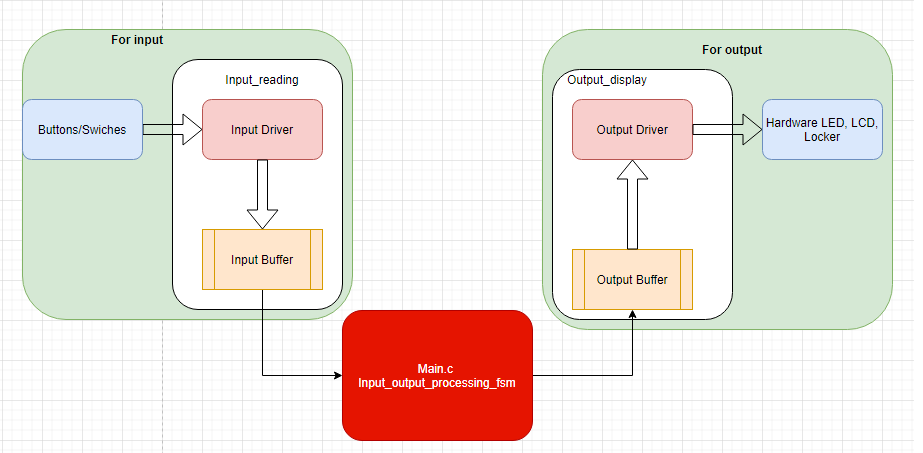
\includegraphics[width=5.5in]{source/picture/bai_3/Input_Output_patterns.png}
    \caption{\textit{Input Output Processing Patterns}}
    \label{bai4_pic_Input_Output_patterns}
\end{figure}

Figure \ref{bai4_pic_Input_Output_patterns} shows that we should have an \emph{input\_reading} module to processing the buttons, then store the processed data to the buffer. Then a module of \emph{input\_output\_processing\_fsm} will process the input data, and update the output buffer. The output driver gets the value from the output buffer to transfer to the hardware. 
\newpage
\subsubsection{Setting up}
\subsubsection{Create a project}
Please follow the instruction in Labs 1 and 2 to create a project that includes: 
\begin{itemize}
    \item PB0 as an input port pin, 
    \item PA0-PA7 as output port pins, and 
    \item Timer 2 10ms interrupt
\end{itemize}

% \begin{figure}[!htp]
%     \centering
%     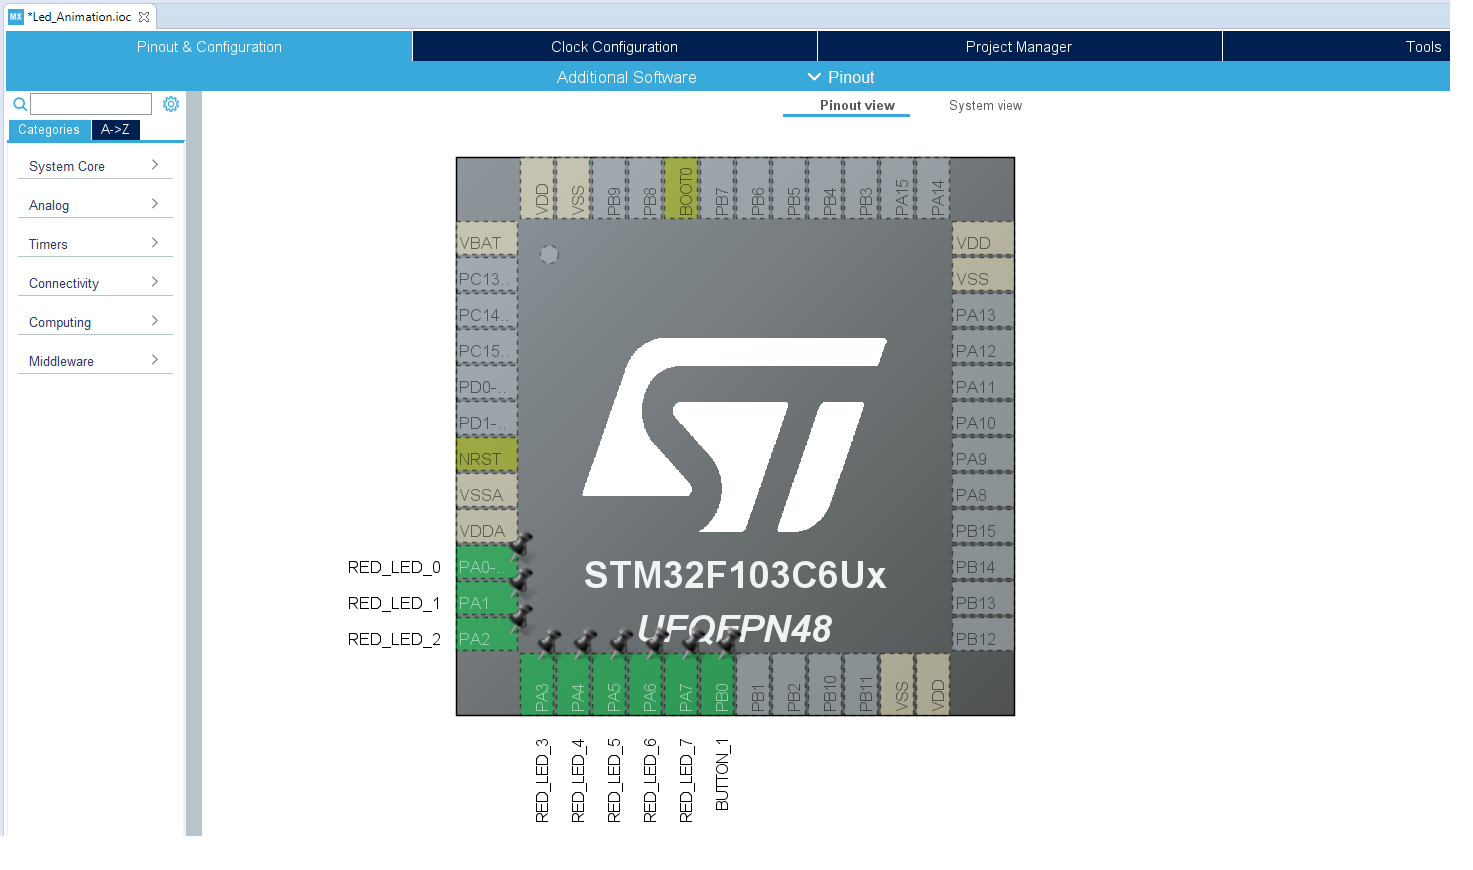
\includegraphics[width=5.5in]{source/picture/bai_3/Input_Output_Settings.png}
%     \caption{\textit{Input Output Setting}}
%     \label{bai4_pic_input_output_setting}
% \end{figure}


\subsubsection{Create a file C source file and header file for input reading}
We are expected to have files for button processing and led display as shown in Figure \ref{bai4_pic_Adding_new_files_to_project}.

\begin{figure}[!htp]
    \centering
    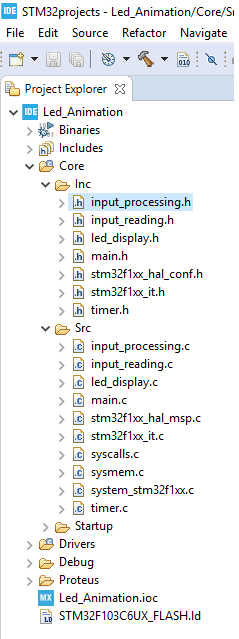
\includegraphics[width=1.5in]{source/picture/bai_3/Adding_new_files_to_project.png}
    \caption{\textit{File Organization}}
    \label{bai4_pic_Adding_new_files_to_project}
\end{figure}

Steps 1 (Figure \ref{bai4_pic_Adding_new_files_to_project_step_1}): Right click to the folder \textbf{Src}, select \textbf{New}, then select \textbf{Source File}. There will be a pop-up. Please type the file name, then click \textbf{Finish}.
\begin{figure}[!htp]
    \centering
    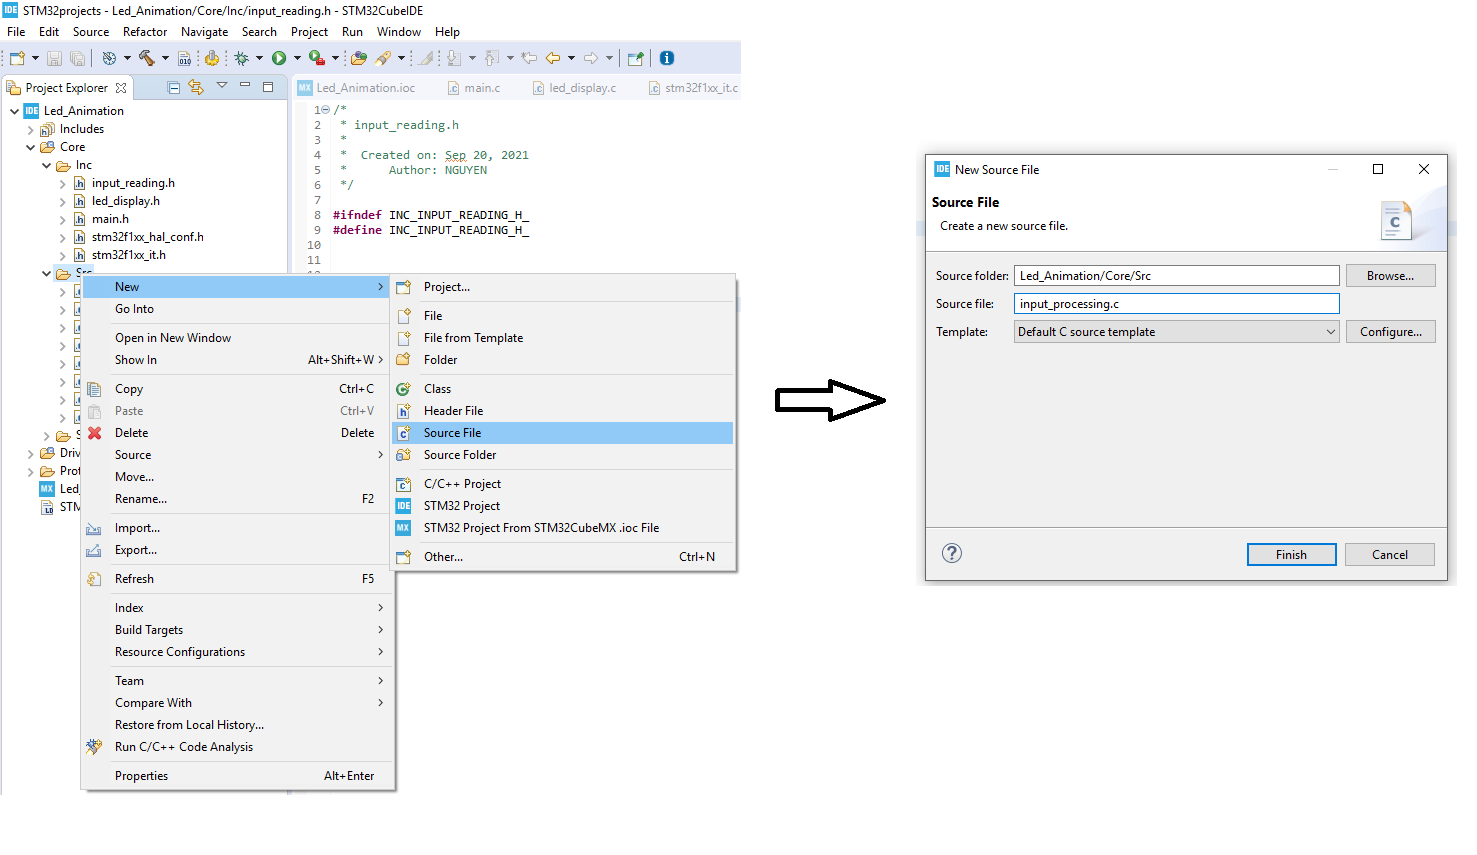
\includegraphics[width=5.5in]{source/picture/bai_3/Adding_new_files_to_project_step_1.png}
    \caption{\textit{Step 1: Create a C source file for input reading}}
    \label{bai4_pic_Adding_new_files_to_project_step_1}
\end{figure}

Step 2 (Figure \ref{bai4_pic_Adding_new_files_to_project_step_3}): Do the same for the C header file in the folder \textbf{Inc}.
\begin{figure}[!htp]
    \centering
    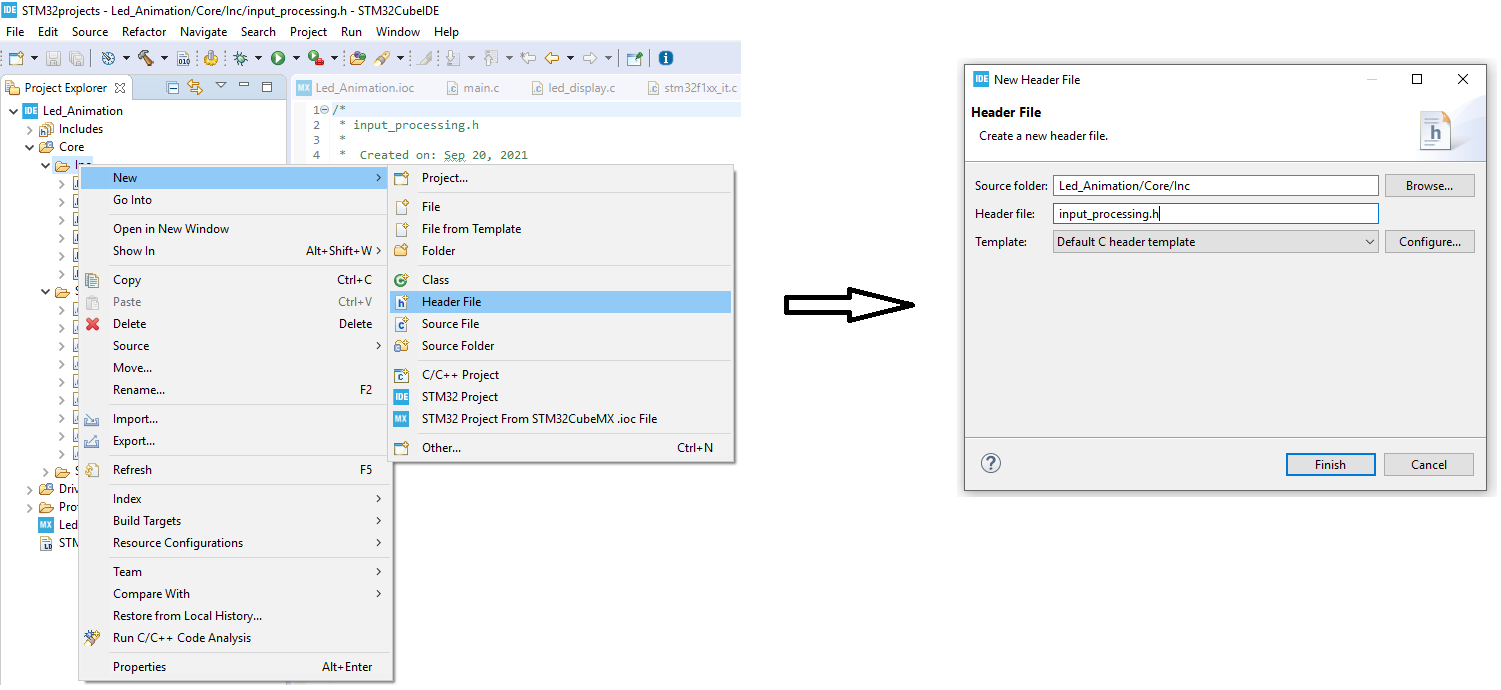
\includegraphics[width=5.5in]{source/picture/bai_3/Adding_new_files_to_project_step_3.png}
    \caption{\textit{Step 2: Create a C header file for input processing}}
    \label{bai4_pic_Adding_new_files_to_project_step_3}
\end{figure}


\newpage

\newpage
\subsubsection{Code For Read Port Pin and Debouncing}
\subsubsection{The code in the input\_reading.c file}
\begin{lstlisting}[caption=Define constants buffers and button\_reading function,language=C++]
#include "main.h"
//we aim to work with more than one buttons
#define N0_OF_BUTTONS 				       1
//timer interrupt duration is 10ms, so to pass 1 second, 
//we need to jump to the interrupt service routine 100 time
#define DURATION_FOR_AUTO_INCREASING	   100
#define BUTTON_IS_PRESSED                  GPIO_PIN_RESET
#define BUTTON_IS_RELEASED                 GPIO_PIN_SET
//the buffer that the final result is stored after 
//debouncing
static GPIO_PinState buttonBuffer[N0_OF_BUTTONS];
//we define two buffers for debouncing
static GPIO_PinState debounceButtonBuffer1[N0_OF_BUTTONS];
static GPIO_PinState debounceButtonBuffer2[N0_OF_BUTTONS];
//we define a flag for a button pressed more than 1 second.
static uint8_t flagForButtonPress1s[N0_OF_BUTTONS];
//we define counter for automatically increasing the value 
//after the button is pressed more than 1 second.
static uint16_t counterForButtonPress1s[N0_OF_BUTTONS];
void button_reading(void){
	for(char i = 0; i < N0_OF_BUTTONS; i ++){
		debounceButtonBuffer2[i] =debounceButtonBuffer1[i];
		debounceButtonBuffer1[i] = HAL_GPIO_ReadPin(BUTTON_1_GPIO_Port, BUTTON_1_Pin);
		if(debounceButtonBuffer1[i] == debounceButtonBuffer2[i])
			buttonBuffer[i] = debounceButtonBuffer1[i];
			if(buttonBuffer[i] == BUTTON_IS_PRESSED){
			//if a button is pressed, we start counting
				if(counterForButtonPress1s[i] < DURATION_FOR_AUTO_INCREASING){
					counterForButtonPress1s[i]++;
				} else {
				//the flag is turned on when 1 second has passed 
				//since the button is pressed.
					flagForButtonPress1s[i] = 1;
					//todo
				}
			} else {
				counterForButtonPress1s[i] = 0;
				flagForButtonPress1s[i] = 0;
			}
	}
}
\end{lstlisting}

% The program reads all buttons two consecutive times and compare the values. If the values are the same, update the value to buttonBuffer. This function should be called inside the timer interrupt service routine.
% \begin{lstlisting}[caption=Read port pin and deboucing,language=C]
% void button_reading(void){
% 	for(char i = 0; i < N0_OF_BUTTONS; i ++){
% 		debounceButtonBuffer2[i] =debounceButtonBuffer1[i];
% 		debounceButtonBuffer1[i] = HAL_GPIO_ReadPin(BUTTON_1_GPIO_Port, BUTTON_1_Pin);
% 		if(debounceButtonBuffer1[i] == debounceButtonBuffer2[i])
% 			buttonBuffer[i] = debounceButtonBuffer1[i];
% 			if(buttonBuffer[i] == BUTTON_IS_PRESSED){
% 			//if a button is pressed, we start counting
% 				if(counterForButtonPress1s[i] < DURATION_FOR_AUTO_INCREASING){
% 					counterForButtonPress1s[i]++;
% 				} else {
% 				//the flag is turned on when 1 second has passed 
% 				//since the button is pressed.
% 					flagForButtonPress1s[i] = 1;
% 					//todo
% 				}

% 			} else {
% 				counterForButtonPress1s[i] = 0;
% 				flagForButtonPress1s[i] = 0;
% 			}
% 	}
% }
% \end{lstlisting}


\begin{lstlisting}[caption=Checking a button is pressed or not,language=C]
unsigned char is_button_pressed(uint8_t index){
	if(index >= N0_OF_BUTTONS) return 0;
	return (buttonBuffer[index] == BUTTON_IS_PRESSED);
}
\end{lstlisting}
\begin{lstlisting}[caption=Checking a button is pressed more than a second or not,language=C]
unsigned char is_button_pressed_1s(unsigned char index){
	if(index >= N0_OF_BUTTONS) return 0xff;
	return (flagForButtonPress1s[index] == 1);
}
\end{lstlisting}
\subsubsection{The code in the input\_reading.h file}
\begin{lstlisting}[caption=Prototype in input\_reading.h file,language=C]
#ifndef INC_INPUT_READING_H_
#define INC_INPUT_READING_H_
void button_reading(void);
unsigned char is_button_pressed(unsigned char index);
unsigned char is_button_pressed_1s(unsigned char index);
#endif /* INC_INPUT_READING_H_ */
\end{lstlisting}

\subsubsection{The code in the timer.c file}
\begin{lstlisting}[caption=Timer interrupt callback function,language=C]
#include "main.h"
#include "input_reading.h"

void HAL_TIM_PeriodElapsedCallback(TIM_HandleTypeDef *htim)
{
	if(htim->Instance == TIM2){
		button_reading();
	}
}

\end{lstlisting}



\newpage
\subsubsection{Button State Processing}
\subsubsection {Finite State Machine}
To solve the example problem, we define 3 states as follows:
\begin{itemize}
    \item State 0: The button is released or the button is in the initial state. 
    \item State 1: When the button is pressed, the FSM will change to State 1 that is increasing the values of PORTA by one value. If the button is released, the FSM goes back to State 0.
    \item State 2: while the FSM is in State 1, the button is kept pressing more than 1 second, the state of FSM will change from 1 to 2. In this state, if the button is kept pressing, the value of PORTA will be increased automatically in every 500ms. If the button is released, the FSM goes back to State 0.
\end{itemize}
\begin{figure}[!htp]
    \centering
    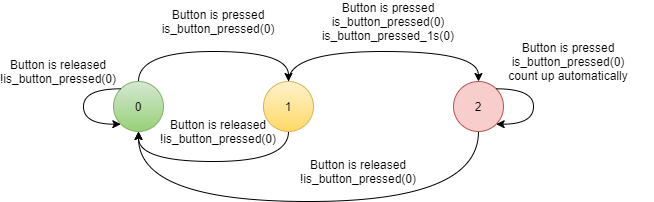
\includegraphics[width=5.5in]{source/picture/bai_3/fsm.png}
    \caption{\textit{An FSM for processing a button}}
    \label{bai4_pic_fsm_for_button_processing}
\end{figure}
\newpage
\subsubsection{The code for the FSM in the input\_processing.c file}
Please note that \emph{fsm\_for\_input\_processing} function should be called inside the super loop of the main functin. 
\begin{lstlisting}[caption=The code in the input\_processing.c file,language=C]
#include "main.h"
#include "input_reading.h"

enum ButtonState{BUTTON_RELEASED, BUTTON_PRESSED, BUTTON_PRESSED_MORE_THAN_1_SECOND} ;
enum ButtonState buttonState = BUTTON_RELEASED;
void fsm_for_input_processing(void){
	switch(buttonState){
	case BUTTON_RELEASED:
		if(is_button_pressed(0)){
			buttonState = BUTTON_PRESSED;
			//INCREASE VALUE OF PORT A BY ONE UNIT
		}
		break;
	case BUTTON_PRESSED:
		if(!is_button_pressed(0)){
			buttonState = BUTTON_RELEASED;
		} else {
			if(is_button_pressed_1s(0)){
				buttonState = BUTTON_PRESSED_MORE_THAN_1_SECOND;
			}
		}
		break;
	case BUTTON_PRESSED_MORE_THAN_1_SECOND:
		if(!is_button_pressed(0)){
			buttonState = BUTTON_RELEASED;
		}
		//todo
		break;
	}
}
\end{lstlisting}
\subsubsection{The code in the input\_processing.h}
\begin{lstlisting}[caption=Code in the input\_processing.h file,language=C]
#ifndef INC_INPUT_PROCESSING_H_
#define INC_INPUT_PROCESSING_H_

void fsm_for_input_processing(void);

#endif /* INC_INPUT_PROCESSING_H_ */
\end{lstlisting}


\subsubsection{The code in the main.c file}
\begin{lstlisting}[caption=The code in the main.c file,language=C]
#include "main.h"
#include "input_processing.h"
//don't modify this part
int main(void){
    HAL_Init();
    /* Configure the system clock */
    SystemClock_Config();
    /* Initialize all configured peripherals */
    MX_GPIO_Init();
    MX_TIM2_Init();
    while (1)
    {
        //you only need to add the fsm function here
        fsm_for_input_processing();
    }
}
\end{lstlisting}

\newpage
\subsection{Exercises and Report}
\subsubsection{Specifications}
You are required to build an application of a traffic light in a cross road which includes some features as described below:
\begin{itemize}
    \item The application has 12 LEDs including 4 red LEDs, 4 amber LEDs, 4 green LEDs.
    \item The application has 4 seven segment LEDs to display time with 2 for each road. The 2 seven segment LEDs will show time for each color LED corresponding to each road.
    \item The application has three buttons which are used
    \subitem - to select modes, 
    \subitem - to modify the time for each color led on the fly, and 
    \subitem - to set the chosen value. 
    \item The application has at least 4 modes which is controlled by the first button. Mode 1 is a normal mode, while modes 2 3 4 are  modification modes. You can press the first button to change the mode. Modes will change from 1 to 4 and back to 1 again. 
    
    \textbf{Mode 1 - Normal mode}: 
    \subitem - The traffic light application is running normally.   
    
    \textbf{Mode 2 - Modify time duration for the red LEDs}: This mode allows you to change the time duration of the red LED in the main road. The expected behaviours of this mode include:  
    \subitem - All single red LEDs are blinking in 2 Hz. 
    \subitem - Use two seven-segment LEDs to display the value.
    \subitem - Use the other two seven-segment LEDs to display the mode.
    \subitem - The second button is used to increase the time duration value for the red LEDs. 
    \subitem - The value of time duration is in a range of 1 - 99. 
    \subitem - The third button is used to set the value.
    
    
    \textbf{Mode 3 - Modify time duration for the amber LEDs}: Similar for the red LEDs described above with the amber LEDs.
    
    
    \textbf{Mode 4 - Modify time duration for the green LEDs}: Similar for the red LEDs described above with the green LEDs.
\end{itemize}

\newpage
\subsection*{Exercise 1: Sketch an FSM}

\noindent\textbf{1. Traffic-Phase FSM (Mode 1 --- Normal Mode)} \\
\small The normal traffic cycle continuously repeats 4 phases: $\text{Start} \longrightarrow S_0 \longrightarrow S_1 \longrightarrow S_2 \longrightarrow S_3 \longrightarrow S_0$. Pressing the \texttt{MODE} button at any state halts the cycle and transitions to Mode 2 for duration configuration.

\vspace{-0.25cm}
\begin{figure}[H]
\centering
\begin{tikzpicture}[node distance=1.5cm and 4.2cm]

    % 4 State circular nodes
    \node[s_green] (S0) {$S_0$};
    \node[s_amber, right=of S0] (S1) {$S_1$};
    \node[s_amber, below=of S0] (S3) {$S_3$};
    \node[s_green, right=of S3] (S2) {$S_2$};

    % Start / Reset
    \node[left=0.8cm of S0, font=\scriptsize\bfseries, align=center] (start) {Start /\\Reset};
    \draw[fsm_edge] (start) -- (S0);

    % Main state transitions
    \draw[fsm_edge] (S0) -- node[above, t_label] {timeout green\\(H: Amber, V: Red)} (S1);
    \draw[fsm_edge] (S1) -- node[right, t_label] {timeout amber\\(H: Red, V: Green)} (S2);
    \draw[fsm_edge] (S2) -- node[below, t_label] {timeout green\\(H: Red, V: Amber)} (S3);
    \draw[fsm_edge] (S3) -- node[left, t_label] {timeout amber\\(H: Green, V: Red)} (S0);

    % Transition to Mode 2
    \node[circle, draw=red!70, dashed, fill=red!10, minimum size=1.0cm, font=\scriptsize\bfseries, align=center]
          at ($(S0)!0.5!(S2)$) (M2_mid) {MODE 2\\(Edit Red)};
          
    \draw[dash_edge] (S0) -- (M2_mid);
    \draw[dash_edge] (S1) -- (M2_mid);
    \draw[dash_edge] (S2) -- (M2_mid);
    \draw[dash_edge] (S3) -- node[below, font=\tiny, text=red!80!black] {is\_button\_pressed(MODE)} (M2_mid);

\end{tikzpicture}
\vspace{-0.4cm}
\caption{Traffic-phase FSM diagram in Mode 1.}
\end{figure}

\vspace{-0.35cm}
\noindent\textbf{7-Segment Display Output per Road Direction (Mode 1):}
\begin{center}
\footnotesize
\begin{tabularx}{\textwidth}{@{}cccp{2.4cm}X@{}}
\toprule
\textbf{State} & \textbf{Horizontal} & \textbf{Vertical} & \textbf{Duration} & \textbf{7-Segment Countdown Value} \\ \midrule
$S_0$ & Green & Red & Green time & Horizontal: green remaining; Vertical: red remaining ($t_{\text{green}} + t_{\text{amber}}$) \\
$S_1$ & Amber & Red & Amber time & Both directions display remaining amber time \\
$S_2$ & Red & Green & Green time & Horizontal: red remaining ($t_{\text{green}} + t_{\text{amber}}$); Vertical: green remaining \\
$S_3$ & Red & Amber & Amber time & Both directions display remaining amber time \\ \bottomrule
\end{tabularx}
\end{center}

\vspace{-0.15cm}
\noindent\textbf{2. Mode-Control and Configuration FSM} \\
\small Includes 4 modes: Mode 1 (normal operation) and Modes 2, 3, 4 (editing Red, Amber, and Green durations). Selected color LEDs blink at 2~Hz. Two digits display the set value ($1 \div 99$), and the other two display the mode index.

\vspace{-0.25cm}
\begin{figure}[H]
\centering
\begin{tikzpicture}[node distance=1.5cm and 4.2cm]

    % 4 Mode circular nodes
    \node[s_blue] (M1) {\textbf{M1}};
    \node[s_red, right=of M1] (M2) {\textbf{M2}};
    \node[s_green, below=of M1] (M4) {\textbf{M4}};
    \node[s_amber, right=of M4] (M3) {\textbf{M3}};

    % Mode Subtitles
    \node[above=1pt of M1, font=\tiny\bfseries] {Normal};
    \node[above=1pt of M2, font=\tiny\bfseries] {Edit RED};
    \node[below=1pt of M3, font=\tiny\bfseries] {Edit AMBER};
    \node[below=1pt of M4, font=\tiny\bfseries] {Edit GREEN};

    % Cyclic MODE transitions
    \draw[fsm_edge] (M1) -- node[above, t_label] {is\_button\_pressed(MODE)} (M2);
    \draw[fsm_edge] (M2) -- node[right, t_label] {is\_button\_pressed(MODE)} (M3);
    \draw[fsm_edge] (M3) -- node[below, t_label] {is\_button\_pressed(MODE)} (M4);
    \draw[fsm_edge] (M4) -- node[left, t_label] {is\_button\_pressed(MODE)} (M1);

    % Self-loop INCREASE (1..99)
    \draw[fsm_edge] (M2) edge[out=40, in=85, loop] node[above right=-2pt, t_label] {INC\\(+1)} (M2);
    \draw[fsm_edge] (M3) edge[out=-40, in=-85, loop] node[below right=-2pt, t_label] {INC\\(+1)} (M3);
    \draw[fsm_edge] (M4) edge[out=-140, in=-95, loop] node[below left=-2pt, t_label] {INC\\(+1)} (M4);

    % SET transitions returning to Mode 1 / S0
    \draw[dash_edge, bend right=28] (M2) to node[above, font=\scriptsize, text=red!80!black] {is\_button\_pressed(SET) $\to$ Save \& Return to $S_0$} (M1);
    \draw[dash_edge] (M3) -- node[sloped, above, font=\scriptsize, text=red!80!black] {is\_button\_pressed(SET)} (M1);

\end{tikzpicture}
\vspace{-0.4cm}
\caption{Mode-control and duration-configuration FSM diagram.}
\end{figure}

\subsubsection{Exercise 2: Proteus Schematic}
The completed crossroad circuit contains one STM32F103C6, twelve traffic LEDs (four red, four amber, and four green), four common-anode seven-segment displays, four PNP digit-enable transistors, sixteen resistors, and three push buttons. The twelve LED resistors limit LED current; four base resistors drive the PNP transistors. The circuit also includes the required supply and ground terminals.

The horizontal road signals are connected to PA1--PA3 (red, green, and amber); the vertical road signals use PA4--PA6 (red, amber, and green). The four digit enables use PA7--PA10. The horizontal and vertical segment buses use PB0--PB6 and PB7--PB13, respectively. MODE, INCREASE, and SET use PA11, PA12, and PA13. The buttons are active-low with pull-ups. The common-anode display segments and PNP digit enables are also active-low.

Figure~\ref{lab3_ex2_schematic} presents the complete Proteus schematic used for all later exercises.

\begin{figure}[H]
    \centering
    \IfFileExists{source/picture/bai_3/lab3_ex2.png}
      {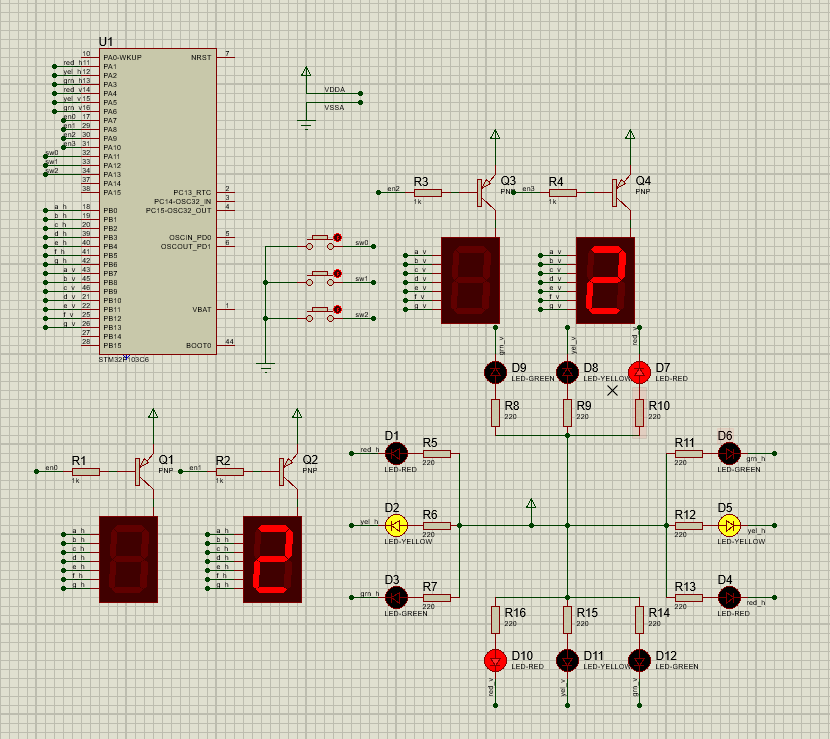
\includegraphics[width=0.98\linewidth]{source/picture/bai_3/lab3_ex2.png}}
      {\fbox{\parbox{0.92\linewidth}{\centering Add the full Proteus schematic here:\\
       \texttt{source/picture/bai\_3/lab3\_ex2.png}}}}
    \caption{Complete Proteus schematic for the crossroad traffic-light controller}
    \label{lab3_ex2_schematic}
\end{figure}

\subsubsection{Exercise 3: Create STM32 Project}
The STM32CubeIDE project targets the STM32F103C6 and uses the HSI clock at 8 MHz. GPIOA and GPIOB are configured to match the schematic in Exercise 2. TIM2 generates the periodic interrupt used by the button reader, display scanner, and software timers.

With an 8 MHz timer clock, the update frequency is
\[
f_{\mathrm{update}} =
\frac{8\,000\,000}{(7999+1)(9+1)} = 100\ \mathrm{Hz},
\]
which gives a 10 ms interrupt interval.

\begin{lstlisting}[caption={TIM2 configuration for a 10 ms interrupt},language=C]
htim2.Instance = TIM2;
htim2.Init.Prescaler = 7999U;
htim2.Init.CounterMode = TIM_COUNTERMODE_UP;
htim2.Init.Period = 9U;
htim2.Init.ClockDivision = TIM_CLOCKDIVISION_DIV1;
if (HAL_TIM_Base_Init(&htim2) != HAL_OK)
{
  Error_Handler();
}

/* Start the periodic interrupt after application initialization. */
HAL_TIM_Base_Start_IT(&htim2);
\end{lstlisting}

The pin assignment and TIM2 settings are shown in the CubeMX captures below.

\begin{figure}[!htp]
    \centering
    \IfFileExists{source/picture/bai_3/lab3_ex3_pin.png}
      {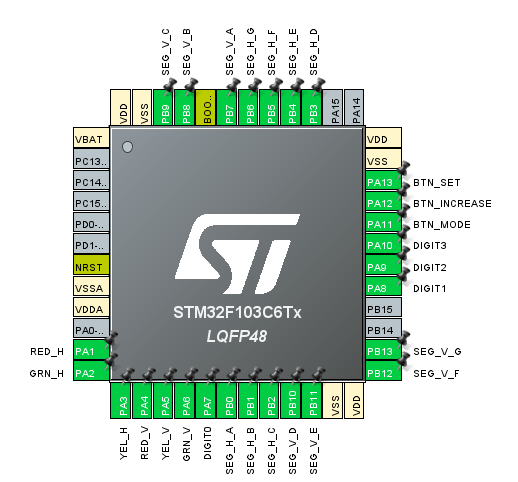
\includegraphics[width=0.67\linewidth]{source/picture/bai_3/lab3_ex3_pin.png}}
      {\fbox{\parbox{0.6\linewidth}{\centering Add the STM32 pin configuration screenshot here:\\
       \texttt{source/picture/bai\_3/lab3\_ex3\_pin.png}}}}
    \hfill
    \IfFileExists{source/picture/bai_3/lab3_ex3_tim.png}
      {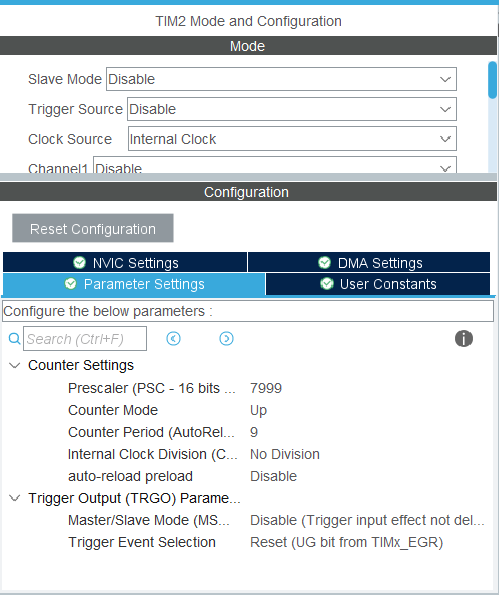
\includegraphics[width=0.30\linewidth]{source/picture/bai_3/lab3_ex3_tim.png}}
      {\fbox{\parbox{0.28\linewidth}{\centering Add the TIM2 settings screenshot here:\\
       \texttt{source/picture/bai\_3/lab3\_ex3\_tim.png}}}}
    \caption{STM32 GPIO pin assignment and TIM2 parameter settings}
    \label{lab3_ex3_ioc}
\end{figure}

\subsubsection{Exercise 4: Modify Timer Parameters}
Exercise 4 compares two TIM2 update intervals by changing \texttt{LAB3\_TIMER\_TICK\_MS}. With an 8 MHz TIM2 clock and prescaler 799, the counter clock is 10 kHz. The auto-reload value is calculated as \texttt{(LAB3\_TIMER\_TICK\_MS * 10U) - 1U}; therefore, a 1 ms tick uses ARR = 9, while a 100 ms tick uses ARR = 999. The screenshots below show both macro selections.

The software timer converts requested delays to hardware ticks by rounding up. Thus, the 250 ms LED blink half-period is 250 ticks with a 1 ms tick, but 3 ticks (300 ms) with a 100 ms tick. The latter setting makes the blink slower because the timer resolution is coarser.

The timer tick and blink half-period are defined separately. Change the tick macro to select either configuration; the TIM2 period follows from the expression in \texttt{main.c}.

\begin{lstlisting}[caption={Selecting the timer tick and application blink interval},language=C]
#define LAB3_TIMER_TICK_MS          1U  /* use 100U for the second case */
#define LAB3_BLINK_HALF_PERIOD_MS 250U
\end{lstlisting}

TIM2 uses a prescaler of 799 and derives its auto-reload value from the selected tick:

\begin{lstlisting}[caption={TIM2 prescaler and auto-reload calculation},language=C]
htim2.Init.Prescaler = 799U;
htim2.Init.Period = (LAB3_TIMER_TICK_MS * 10U) - 1U;
\end{lstlisting}

The blink behavior can be demonstrated in the Exercise 6 or Exercise 10 simulation video.

\begin{figure}[!htp]
    \centering
    \IfFileExists{source/picture/bai_3/lab3_ex4_tick1.png}
      {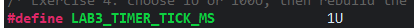
\includegraphics[width=0.47\linewidth]{source/picture/bai_3/lab3_ex4_tick1.png}}
      {\fbox{\parbox{0.43\linewidth}{\centering Add the 1 ms tick macro screenshot:\\
       \texttt{source/picture/bai\_3/lab3\_ex4\_tick1.png}}}}
    \hfill
    \IfFileExists{source/picture/bai_3/lab3_ex4_tick100.png}
      {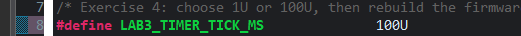
\includegraphics[width=0.47\linewidth]{source/picture/bai_3/lab3_ex4_tick100.png}}
      {\fbox{\parbox{0.43\linewidth}{\centering Add the 100 ms tick macro screenshot:\\
       \texttt{source/picture/bai\_3/lab3\_ex4\_tick100.png}}}}
    \caption{Source selections for 1 ms and 100 ms timer ticks}
    \label{lab3_ex4_timer}
\end{figure}

\subsubsection{Exercise 5: Adding code for button debouncing}
The input and display functions are separated into reusable modules. Button input and debouncing are implemented in \texttt{Core/Inc/button.h} and \texttt{Core/Src/button.c}. Seven-segment output is implemented in \texttt{Core/Inc/seven\_segment.h} and \texttt{Core/Src/seven\_segment.c}. The application calls these modules from \texttt{traffic\_app.c}; the timer interrupt samples the buttons and refreshes the multiplexed displays.

The three active-low buttons are sampled once per timer tick. Each switch connects its input to ground when pressed, so the GPIO reads low. A state change is accepted only after two consecutive matching samples; this filters short switch bounces. A valid press is then queued as one event for the main loop.

In the circuit shown in Figure~\ref{lab3_ex5_buttons}, \texttt{sw0} is MODE, \texttt{sw1} is INCREASE, and \texttt{sw2} is SET. MODE cycles through Normal, Red edit, Amber edit, Green edit, and back to Normal. INCREASE adds one to the currently selected duration in an editing mode; it has no effect in Normal mode. SET leaves an editing mode and resumes the traffic cycle with the current values; it has no effect in Normal mode.

\begin{lstlisting}[caption={Button debounce and press-event generation},language=C]
if (sample == buttons[i].raw_state)
{
  if (buttons[i].stable_samples < LAB3_BUTTON_DEBOUNCE_SAMPLES)
    buttons[i].stable_samples++;
}
else
{
  buttons[i].raw_state = sample;
  buttons[i].stable_samples = 1U;
}

if (buttons[i].stable_samples >= LAB3_BUTTON_DEBOUNCE_SAMPLES &&
    buttons[i].stable_state != buttons[i].raw_state)
{
  buttons[i].stable_state = buttons[i].raw_state;
  if (buttons[i].stable_state == GPIO_PIN_RESET)
    press_events |= (uint8_t)(1U << i);
}
\end{lstlisting}

The debounce configuration is \texttt{LAB3\_BUTTON\_DEBOUNCE\_SAMPLES = 2}. The following application code shows how the first button advances the mode after debouncing:

\begin{lstlisting}[caption={Advancing the mode on a debounced MODE press},language=C]
if (button_take_press(BUTTON_MODE) != 0U)
{
  if (mode == MODE_NORMAL) enter_edit(MODE_RED);
  else if (mode == MODE_RED) enter_edit(MODE_AMBER);
  else if (mode == MODE_AMBER) enter_edit(MODE_GREEN);
  else enter_normal();
  return;
}
\end{lstlisting}

The demonstration clip shows the buttons being used and the debounced response: \href{https://github.com/quangnguyencomeng/CO3009-261-CC-2453052/blob/main/Lab/lab_reports/source/vids/lab3_ex5.mp4}{Exercise 5 demonstration video}.

\begin{figure}[!htp]
    \centering
    \IfFileExists{source/picture/bai_3/lab3_ex5.png}
      {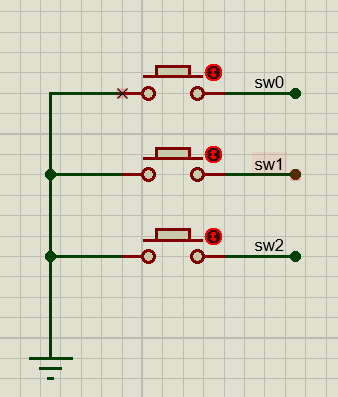
\includegraphics[width=0.55\linewidth]{source/picture/bai_3/lab3_ex5.png}}
      {\fbox{\parbox{0.52\linewidth}{\centering Add the three-button circuit image here:\\
       \texttt{source/picture/bai\_3/lab3\_ex5.png}}}}
    \caption{Active-low MODE, INCREASE, and SET buttons}
    \label{lab3_ex5_buttons}
\end{figure}

\newpage
\subsubsection{Exercise 6: Adding code for displaying modes}
Modes 2, 3, and 4 edit red, amber, and green durations. The selected color LEDs blink with a 250 ms on/off half-period (2 Hz). The first two digits show the selected duration; the other two show the mode number. The four common-anode displays are multiplexed as two independent road pairs.

\begin{lstlisting}[caption={Rendering an editing mode},language=C]
static void render_edit(void)
{
  TrafficColour colour = edited_colour();
  uint8_t value = durations[colour];

  traffic_led_all_off();
  if (blink_on != 0U)
    traffic_led_set_mask(colour, 0x0FU);

  seven_segment_set_values((int8_t)(value / 10U),
                           (int8_t)(value % 10U),
                           0, (int8_t)mode);
}
\end{lstlisting}

The four circuit captures below show the normal traffic output and the selected-color indication in Modes 2--4. The videos demonstrate INCREASE behavior in two ways: \href{https://github.com/quangnguyencomeng/CO3009-261-CC-2453052/blob/main/Lab/lab_reports/source/vids/lab3_ex6_increase_step_by_step.mp4}{increase once per button press} and \href{https://github.com/quangnguyencomeng/CO3009-261-CC-2453052/blob/main/Lab/lab_reports/source/vids/lab3_ex6_increase_hold.mp4}{continuous increase while holding the button}.

\begin{figure}[!htp]
    \centering
    \begin{minipage}[t]{0.47\linewidth}\centering
      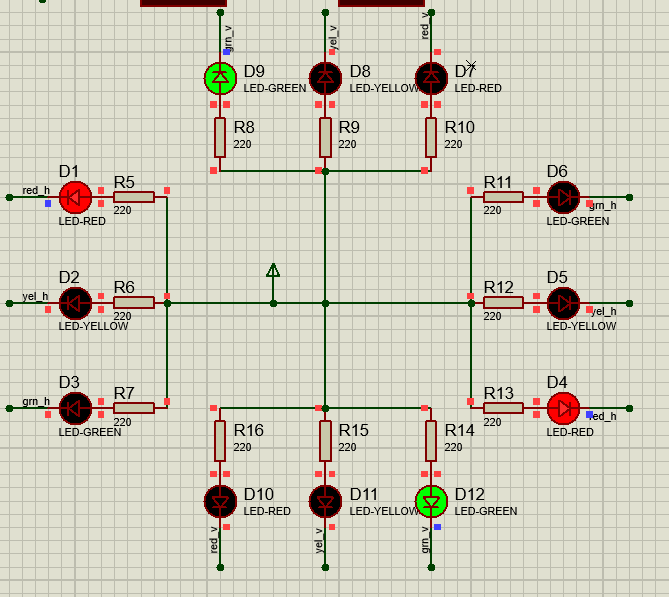
\includegraphics[width=\linewidth]{source/picture/bai_3/lab3_ex6_m1.png}\\
      \small (a) Mode 1: normal traffic operation
    \end{minipage}\hfill
    \begin{minipage}[t]{0.47\linewidth}\centering
      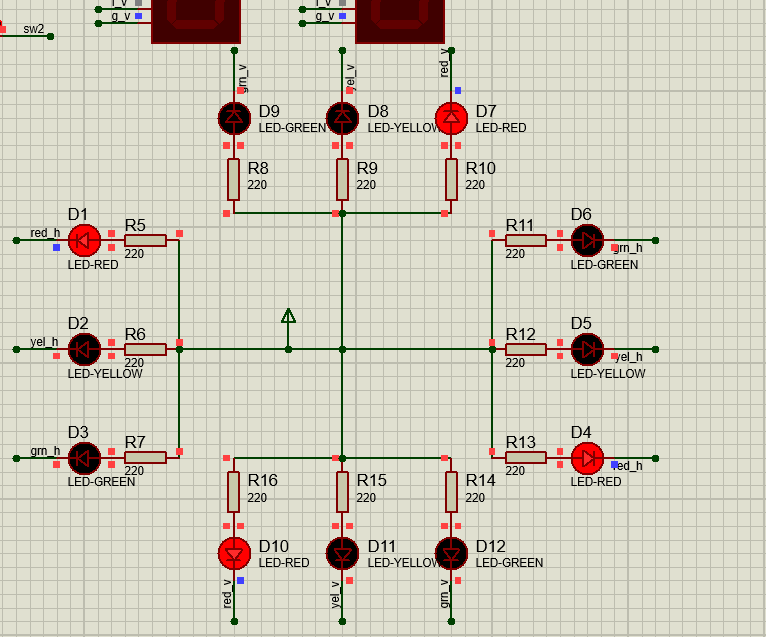
\includegraphics[width=\linewidth]{source/picture/bai_3/lab3_ex6_m2.png}\\
      \small (b) Mode 2: red-duration selection
    \end{minipage}\\[2mm]
    \begin{minipage}[t]{0.47\linewidth}\centering
      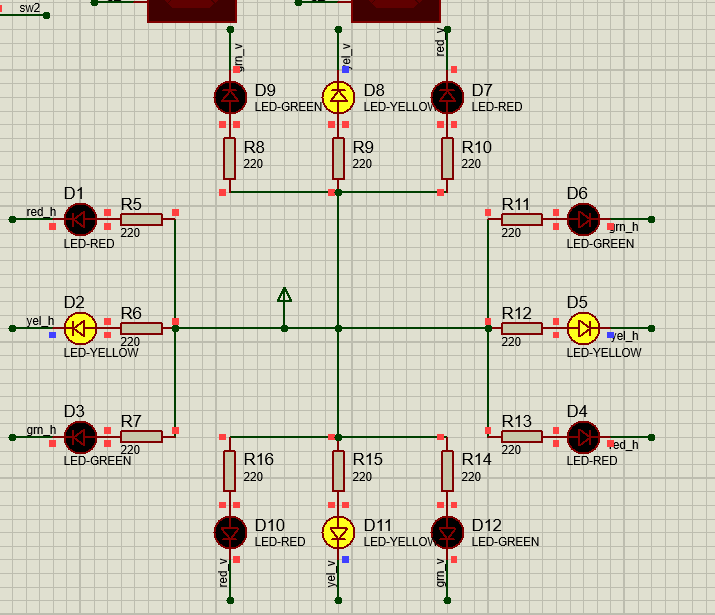
\includegraphics[width=\linewidth]{source/picture/bai_3/lab3_ex6_m3.png}\\
      \small (c) Mode 3: amber-duration selection
    \end{minipage}\hfill
    \begin{minipage}[t]{0.47\linewidth}\centering
      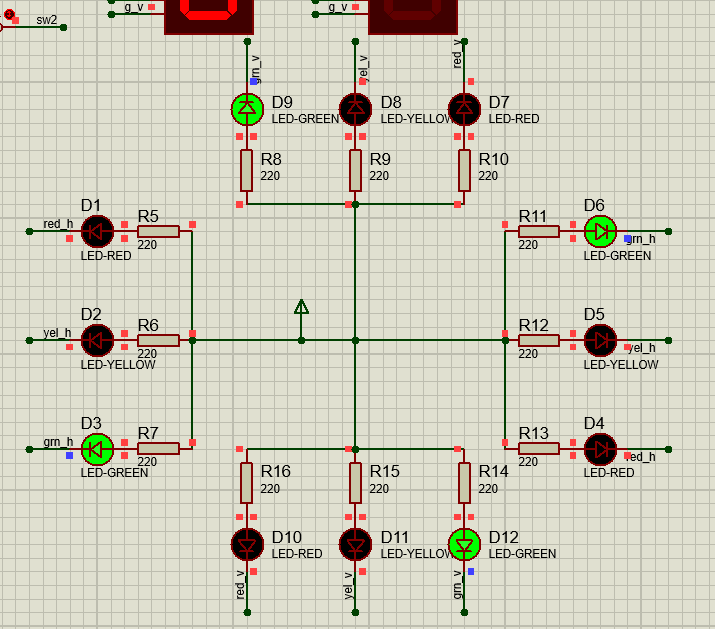
\includegraphics[width=\linewidth]{source/picture/bai_3/lab3_ex6_m4.png}\\
      \small (d) Mode 4: green-duration selection
    \end{minipage}
    \caption{Circuit output in Normal mode and the three duration-editing modes}
    \label{lab3_ex6_mode}
\end{figure}

\subsubsection{Exercise 7: Adding code for increasing time duration value for the red LEDs}
In Mode 2, INCREASE changes the red duration and SET returns to Mode 1 with the chosen value retained during the current run. The general increment code wraps a value above 99 to 1. The red-duration helper also keeps red related to green and amber: when a wrapped candidate would break that relation, the helper recalculates red from the other two durations. Consequently, an increase at the upper boundary can leave the displayed red value unchanged.

\begin{lstlisting}[caption={Increasing the selected duration},language=C]
if (increase_pressed != 0U)
{
  TrafficColour colour = edited_colour();
  durations[colour]++;
  if (durations[colour] > TRAFFIC_MAX_DURATION_SECONDS)
    durations[colour] = TRAFFIC_MIN_DURATION_SECONDS;

  reconcile_durations(colour);
  render_edit();
}
\end{lstlisting}

The video demonstrates the upper-boundary behavior in Mode 2 with amber set to 2 seconds and green set to 3 seconds. When INCREASE is pressed while red is 99 seconds, the increment first produces 100, which wraps to 1. The reconciliation logic then detects that red is not greater than amber and recalculates red as amber plus green, so the displayed red duration returns to 5 seconds. The demonstration is available here: \href{https://github.com/quangnguyencomeng/CO3009-261-CC-2453052/blob/main/Lab/lab_reports/source/vids/lab3_ex7.mp4}{Exercise 7 red-duration upper-boundary video}.

\subsubsection{Exercise 8: Adding code for increasing time duration value for the amber LEDs}
Mode 3 edits the amber duration while keeping the red duration fixed. The green duration is recalculated as red minus amber, so the relation red = amber + green is preserved. For example, with red = 5, amber = 2, and green = 3, two INCREASE presses change amber to 4 and green to 1 while red remains 5. If amber reaches the red value, amber wraps to 1 so that green remains at least 1.

\begin{lstlisting}[caption={Keeping red fixed while amber is edited},language=C]
else if (changed == TRAFFIC_AMBER)
{
  if (amber >= red)
  {
    amber = TRAFFIC_MIN_DURATION_SECONDS;
    durations[TRAFFIC_AMBER] = amber;
  }
  durations[TRAFFIC_GREEN] = red - amber;
}
\end{lstlisting}

The two captures show Mode 3 before and after an INCREASE action: the amber duration changes from 05 to 06. The video demonstrates the adjustment: \href{https://github.com/quangnguyencomeng/CO3009-261-CC-2453052/blob/main/Lab/lab_reports/source/vids/lab3_ex8.mp4}{Exercise 8 amber-duration adjustment video}.

\begin{figure}[!htp]
    \centering
    \begin{minipage}[t]{0.48\linewidth}\centering
      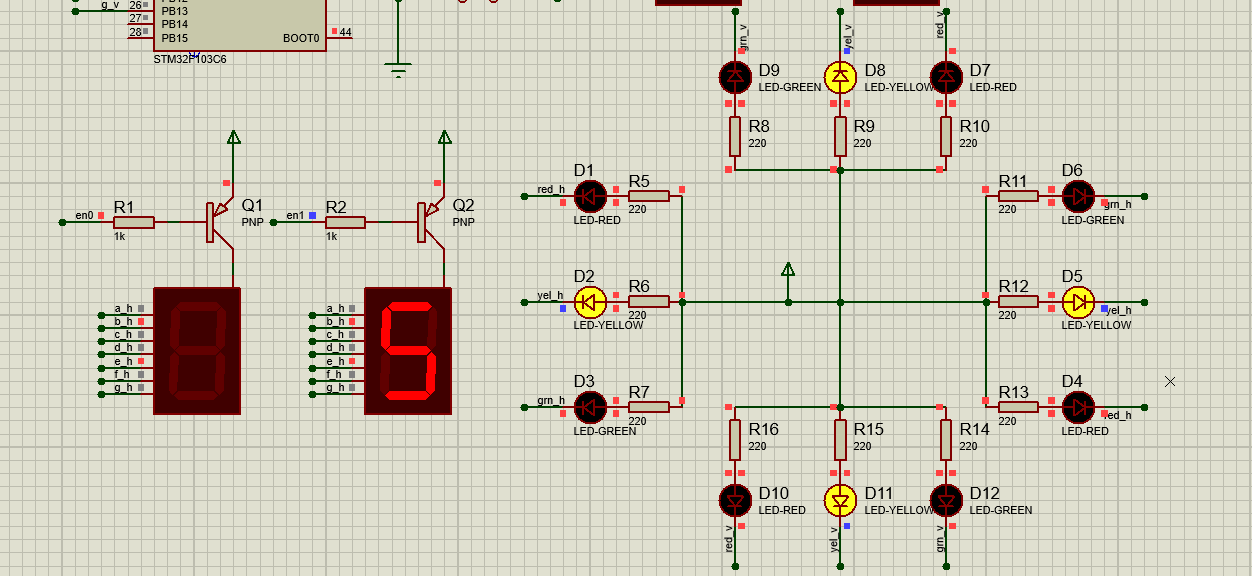
\includegraphics[width=\linewidth]{source/picture/bai_3/lab3_ex8_5.png}\\
      \small (a) Mode 3, amber duration: 05
    \end{minipage}\hfill
    \begin{minipage}[t]{0.48\linewidth}\centering
      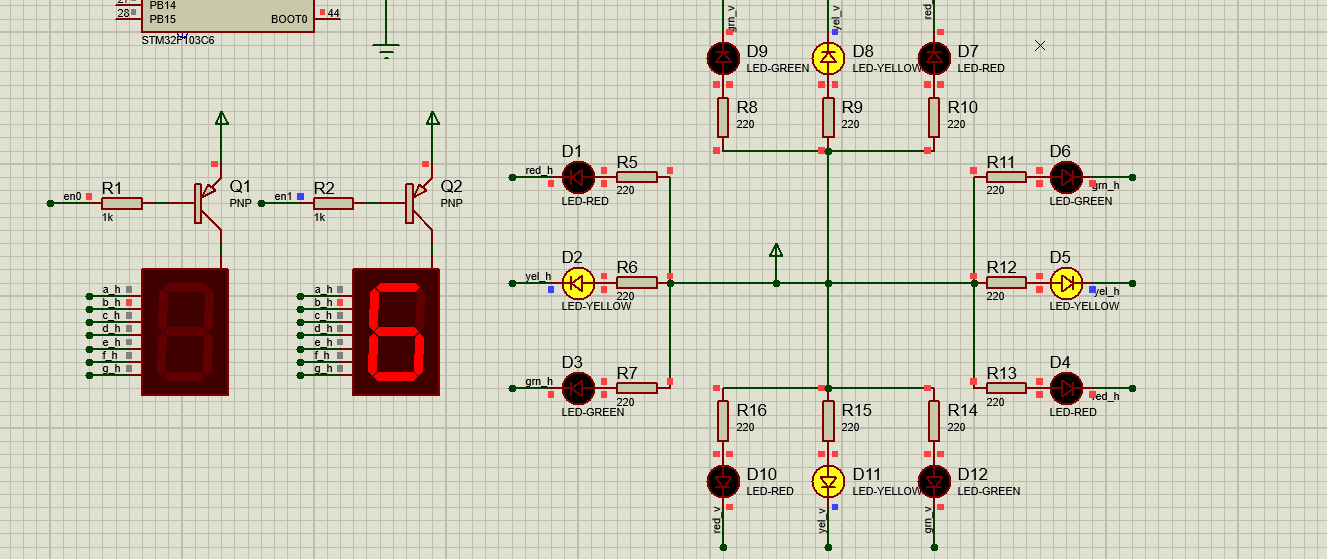
\includegraphics[width=\linewidth]{source/picture/bai_3/lab3_ex8_6.png}\\
      \small (b) Mode 3, amber duration: 06
    \end{minipage}
    \caption{Amber-duration editing before and after increasing the selected value}
    \label{lab3_ex8_amber}
\end{figure}

\subsubsection{Exercise 9: Adding code for increasing time duration value for the green LEDs}
Mode 4 edits the green duration while keeping amber unchanged. After each INCREASE press, a value above 99 wraps to 1, then the red duration is recalculated as green plus amber. If that sum exceeds 99, red is limited to 99.

\begin{lstlisting}[caption={Recomputing red after a green-duration change},language=C]
else
{
  durations[TRAFFIC_RED] = green + amber <= 99U ?
                           green + amber : 99U;
}
\end{lstlisting}

The video demonstrates the upper-boundary sequence with amber fixed at 2 seconds: green increases from 3 to 99, wraps to 1 on the next press, and is then increased to 7. Red is recalculated throughout; at green = 7, red becomes 9 seconds (7 + 2). The demonstration is available here: \href{https://github.com/quangnguyencomeng/CO3009-261-CC-2453052/blob/main/Lab/lab_reports/source/vids/lab3_ex9.mp4}{Exercise 9 green-duration upper-boundary video}.

\begin{figure}[!htp]
    \centering
    \IfFileExists{source/picture/bai_3/lab03_ex09_green.png}
      {\includegraphics[width=0.9\linewidth]{source/picture/bai_3/lab03_ex09_green.png}}
      {\fbox{\parbox{0.84\linewidth}{\centering Add a green-duration editing screenshot here:\\
       \texttt{source/picture/bai\_3/lab03\_ex09\_green.png}}}}
    \caption{Green-duration editing mode}
    \label{lab3_ex9_green}
\end{figure}

\subsubsection{Exercise 10: To finish the project}
Exercise 10 integrates the four-phase traffic controller, button debouncing, mode selection, seven-segment multiplexing, and duration adjustment. In normal operation, the phase sequence repeats as follows:
\[
S_0\ (\text{Horizontal Green, Vertical Red}) \rightarrow
S_1\ (\text{Horizontal Amber, Vertical Red}) \rightarrow
S_2\ (\text{Horizontal Red, Vertical Green}) \rightarrow
S_3\ (\text{Horizontal Red, Vertical Amber}) \rightarrow S_0.
\]
Each phase advances when its timer expires. MODE enters the duration-editing modes; INCREASE changes the selected duration; SET returns to normal operation.

The main loop handles application events while the timer callback services the periodic tasks:

\begin{lstlisting}[caption={Main loop and TIM2 application tick},language=C]
while (1)
{
  traffic_app_run();
}

void HAL_TIM_PeriodElapsedCallback(TIM_HandleTypeDef *htim)
{
  if (htim->Instance == TIM2)
    traffic_app_timer_tick();
}
\end{lstlisting}

The four Proteus captures document the complete phase sequence in order. In every phase, the opposing direction remains red during the other direction's green or amber interval. The integrated demonstration video shows the repeating cycle, editing the red, amber, and green durations, and using SET to return to normal mode: \href{https://github.com/quangnguyencomeng/CO3009-261-CC-2453052/blob/main/Lab/lab_reports/source/vids/lab3_ex10.mp4}{Exercise 10 complete-system demonstration video}.

\begin{figure}[!htp]
    \centering
    \begin{minipage}[t]{0.48\linewidth}\centering
      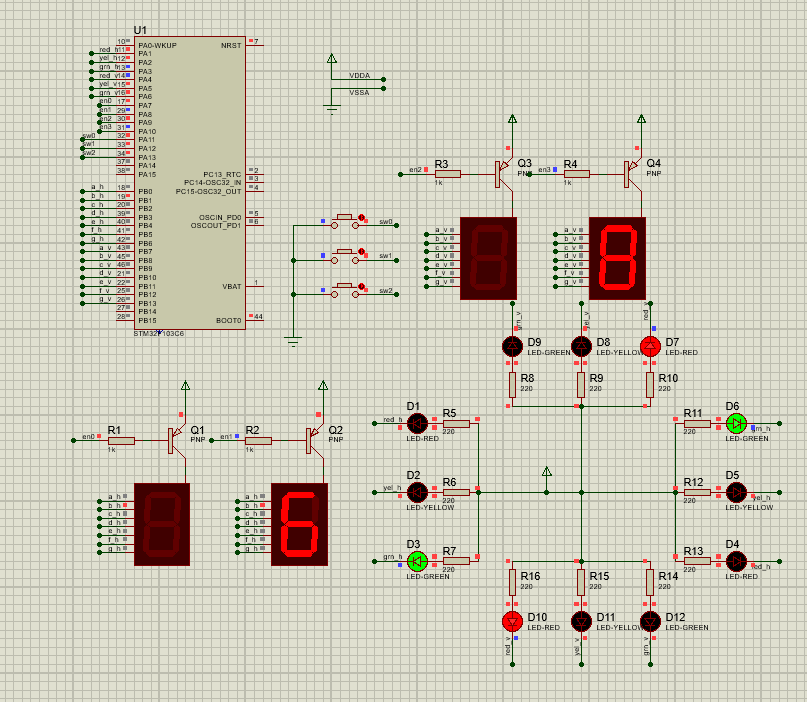
\includegraphics[width=\linewidth]{source/picture/bai_3/lab3_ex10_1.png}\\
      \small (a) Phase $S_0$: horizontal green, vertical red
    \end{minipage}\hfill
    \begin{minipage}[t]{0.48\linewidth}\centering
      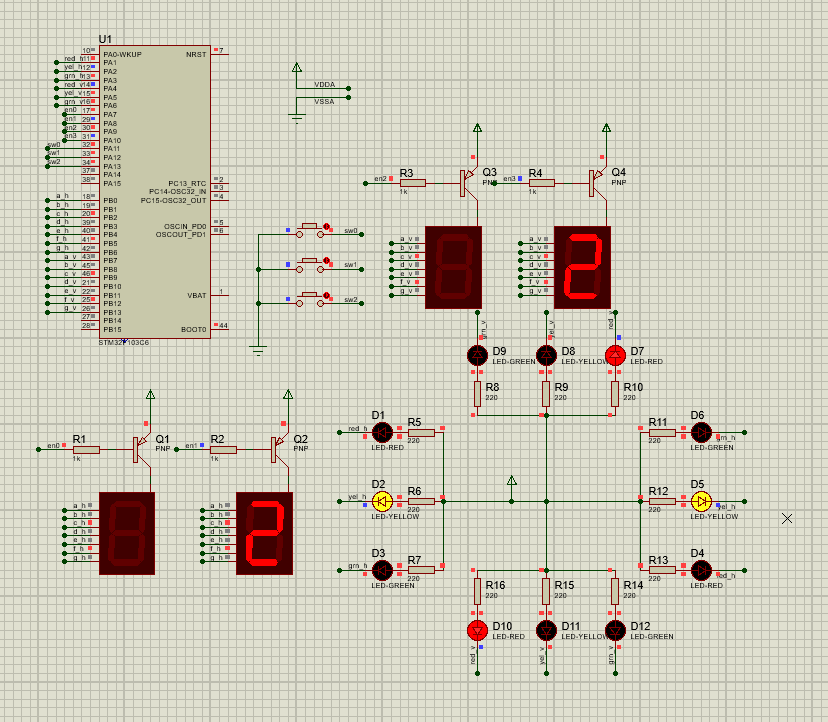
\includegraphics[width=\linewidth]{source/picture/bai_3/lab3_ex10_2.png}\\
      \small (b) Phase $S_1$: horizontal amber, vertical red
    \end{minipage}\\[2mm]
    \begin{minipage}[t]{0.48\linewidth}\centering
      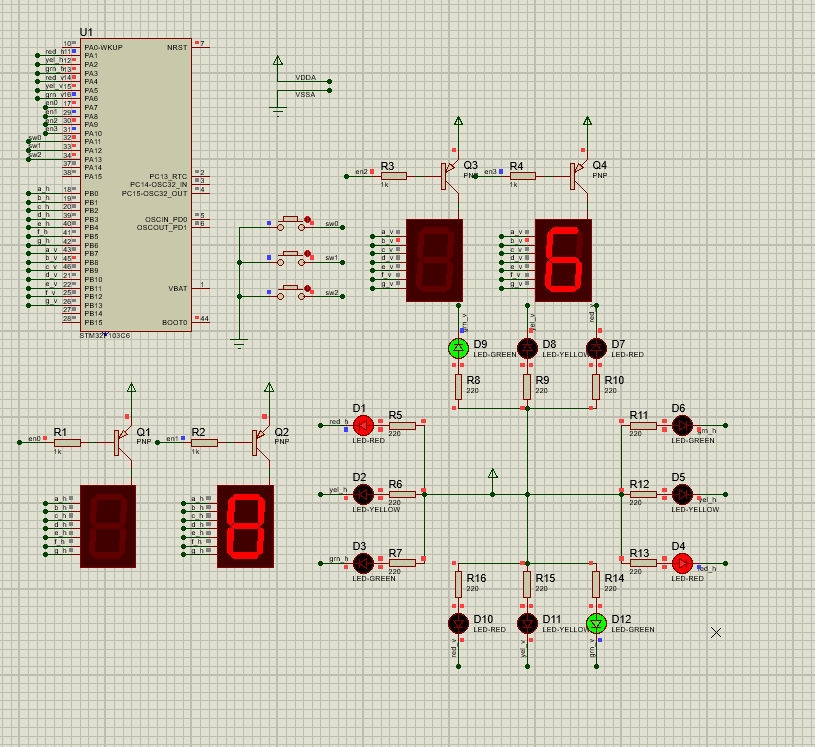
\includegraphics[width=\linewidth]{source/picture/bai_3/lab3_ex10_3.png}\\
      \small (c) Phase $S_2$: horizontal red, vertical green
    \end{minipage}\hfill
    \begin{minipage}[t]{0.48\linewidth}\centering
      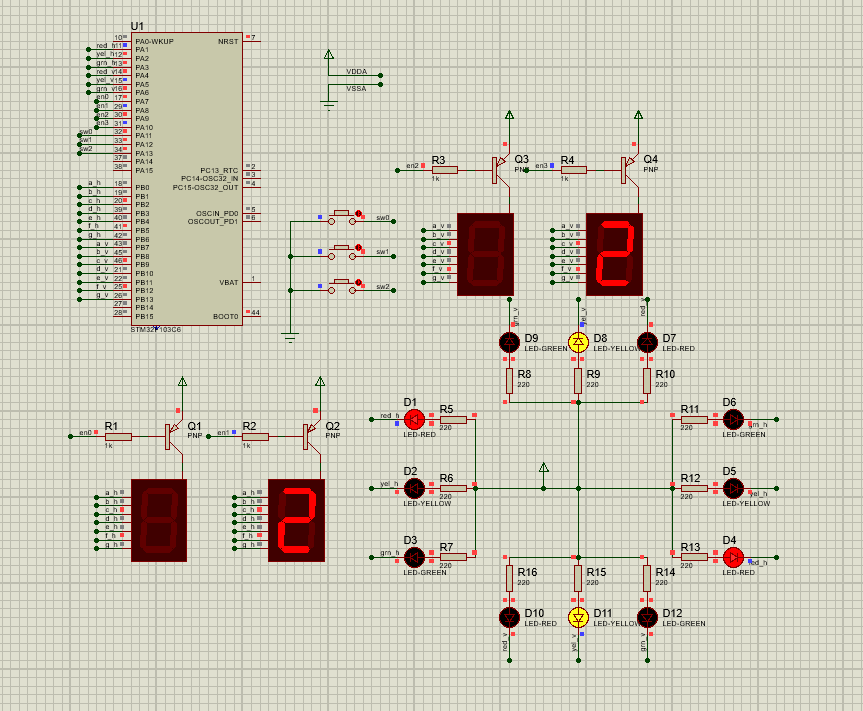
\includegraphics[width=\linewidth]{source/picture/bai_3/lab3_ex10_4.png}\\
      \small (d) Phase $S_3$: horizontal red, vertical amber
    \end{minipage}
    \caption{Integrated traffic-light controller across its four phases, shown in sequence}
    \label{lab3_ex10_phases}
\end{figure}

% \subsection{Problem 1}

% In this week lab, assume you have two button and 8 LEDs, you have to write a program that
% \begin{itemize}
%     \item Has a timer which has an interrupt in every 10 milliseconds.  
%     \item  Reads values of buttons 1 and 2 every 10 milliseconds. The read button function should be called inside the timer interrupt service routine.
%     \item Increases the value of LEDs connected to PORTA when the button 1 is pressed.
%     \item Increases the value of PORTA automatically in every 0.5 second, if the button 1 is pressed in more than 1 second.
%     \item Increases the value of PORTA automatically in every 0.1 second, if the button 1 is pressed in more than 3 seconds.
%     \item Decreases the value of PORTA when the button 2 is pressed
%     \item Decreases the value of PORTA automatically in every 0.5 second, if the button 2 is pressed in more than 1 second.
%     \item Decreases the value of PORTA automatically in every 0.1 second, if the button 2 is pressed in more than 3 seconds.
%     \item The above values such as 10 ms, 0.5 s, 0.1s, 1 s and 3 s are fixed values as an example. Your program, however, needs to provide an easy way to change those values. For example, you should use DEFINE to define those values.
%     \item If both buttons 1 and 2 are pressed, button 1 has a higher priority.
% \end{itemize}


% \subsection{Problem 2 - A digital clock}
%  You have to write a program that mimics a Casio digital watch. Assume you have 2 buttons and 6 seven-segment LED, a program should have
% \begin{itemize}
%     \item A normal clock that shows hours, minutes, and seconds on 6 seven-segment LEDs.
%     \item  A stopwatch that shows minutes, seconds and 1/100 second
%     \item We use button 1 to change modes of a digital watch. Every time button 1 is pressed, the watch will change to the next mode.
%     \item Mode 0: runs normal clock (default)
%     \item Mode 1: modifies hours. In this mode, the hour number is blinking, and button 2 is used for increasing the hour number.  If button 2 is kept pressed more than 1 second, the hour number will increase automatically, i.e., 5 times per second. Please note that the hour number should be returned to 0 when it reaches 23.
%     \item  Mode 2: modifies minutes. Similar to mode 1, the minute number is blinking and increases when button 2 is pressed.
%     \item Mode 3: modifies seconds. Similar to mode 1, the second number is blinking and increases when button 2 is pressed.
%     \item Mode 4: runs a stopwatch. Using button 2 to start and stop the watch.  
 
% \end{itemize}
%  Please note that while the stopwatch is running, the normal clock is still running in the background.


 

% \subsection{Instructions}

% Your task is to sketch an FSM that describes your idea of how to solve the above problems and  writes a firmware that runs on STM32.



 

% \subsection{Submission}

% You need to
% \begin{itemize}
%     \item Demonstrate your work in the lab class and then
%     \item  Submit your FSM sketches and source code to the BKeL.
% \end{itemize}
